% Lecture Template for ME3023 -  Measurements in Mechanical Systems - Tennessee Technological University
% Spring 2020 - Summer 2020 - Fall 2020 - Spring 2021 - Summer 2021 - Fall 2023
% Tristan Hill, May 07, 2020 - June 12, 2020 - July 08, 2020 - Novemeber 02, 2020 - March 28, 2021 - May 25, 2021 - August 21, 2022 - September 02, 2023 - September 09, 2023

% Fall 2023 - condensing and streamlining lectures by combining topics into a single PDF under the module name
%			  this will simplify file and link management as well as make lectures easier to use in class
%			- added image/ to clean directory and reduce redundancy, specific to module for now  

% Module Name: - Sensors
% Topic 1 - Introduction and Overview 
% Topic 2 - IC and MEMs based Sensors
 

\documentclass[fleqn]{beamer} % for presentation (has nav buttons at bottom)
\usepackage{/home/tntech.edu/thill/courses/measurements/lectures/measurements_lectures}
%\usepackage{/home/thill/courses/measurements/lectures/measurements_lectures}
%\usepackage{/mnt/c/Users/thill/Documents/courses/measurements/lectures/measurements_lectures}

\author{ME3023 - Measurements in Mechanical Systems} % original formatting from Mike Renfro, September 21, 2004

\newcommand{\MNUM}{4\hspace{2mm}} % module number 
\newcommand{\moduletitle}{Sensors}

\newcommand{\sectionItitle}{Introduction and Overview}
\newcommand{\sectionIItitle}{IC and MEMS based Sensors}

\newcommand{\sectionIsubsectionItitle}{Analog and Digital Sensors}
\newcommand{\sectionIsubsectionIItitle}{Example 1: Distance or Range}
\newcommand{\sectionIsubsectionIIItitle}{Example 2: Rotation}
\newcommand{\sectionIsubsectionIVtitle}{Example 3: Orientation}

\newcommand{\sectionIIsubsectionItitle}{Integrated Circuits}
\newcommand{\sectionIIsubsectionIItitle}{Micro Electro-Mechanical Devices}
\newcommand{\sectionIIsubsectionIIItitle}{Example 1: Accelerometer}
\newcommand{\sectionIIsubsectionIVtitle}{Example 2: Magnometer and Digital Compass}

\newcommand{\btVFill}{\vskip0pt plus 1filll}

% custom box
\newsavebox{\mybox}

\title{Lecture Module - \moduletitle}

\date{Mechanical Engineering\vspc Tennessee Technological University}

\begin{document}

	\lstset{language=MATLAB,basicstyle=\ttfamily\small,showstringspaces=false}

	\frame{\titlepage \center\begin{framed}\Large \textbf{Module \MNUM - \moduletitle}\end{framed} \vspace{5mm}}

	% Module Outline
	\begin{frame} 
		\large \textbf{Module \MNUM - \moduletitle} \vspace{3mm}\\

		\begin{itemize}
			\item Topic 1 - \hyperlink{sectionI}{\sectionItitle} \vspc % section I
			\item Topic 2 - \hyperlink{sectionII}{\sectionIItitle} \vspc % section II
		\end{itemize}

	\end{frame}

	% section I
	\section{\sectionItitle}\label{sectionI}

		% section I Outline
		\begin{frame} 
			\large \textbf{Topic 1 - \sectionItitle} \vspace{3mm}\\

			\begin{itemize}
				\item \hyperlink{sectionIsubsectionI}{\sectionIsubsectionItitle} \vspc %  section I subsection I
				\item \hyperlink{sectionIsubsectionII}{\sectionIsubsectionIItitle} \vspc % section I subsection II
				\item \hyperlink{sectionIsubsectionIII}{\sectionIsubsectionIIItitle} \vspc % section I subsection III
				\item \hyperlink{sectionIsubsectionIV}{\sectionIsubsectionIVtitle} \vspc % section I subsection IV
			\end{itemize}
		\end{frame}
		
		% section I subsection I 
		\subsection{\sectionIsubsectionItitle}\label{sectionIsubsectionI}

			\begin{frame}
				\frametitle{\sectionIsubsectionItitle}
				
				a {\PR sensor}, a physical element that employs some natural phenomenon... ...to sense the variable being measured
	
				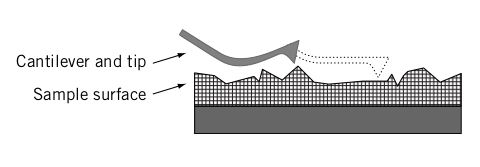
\includegraphics[scale=0.30]{images/sensor_stage.png}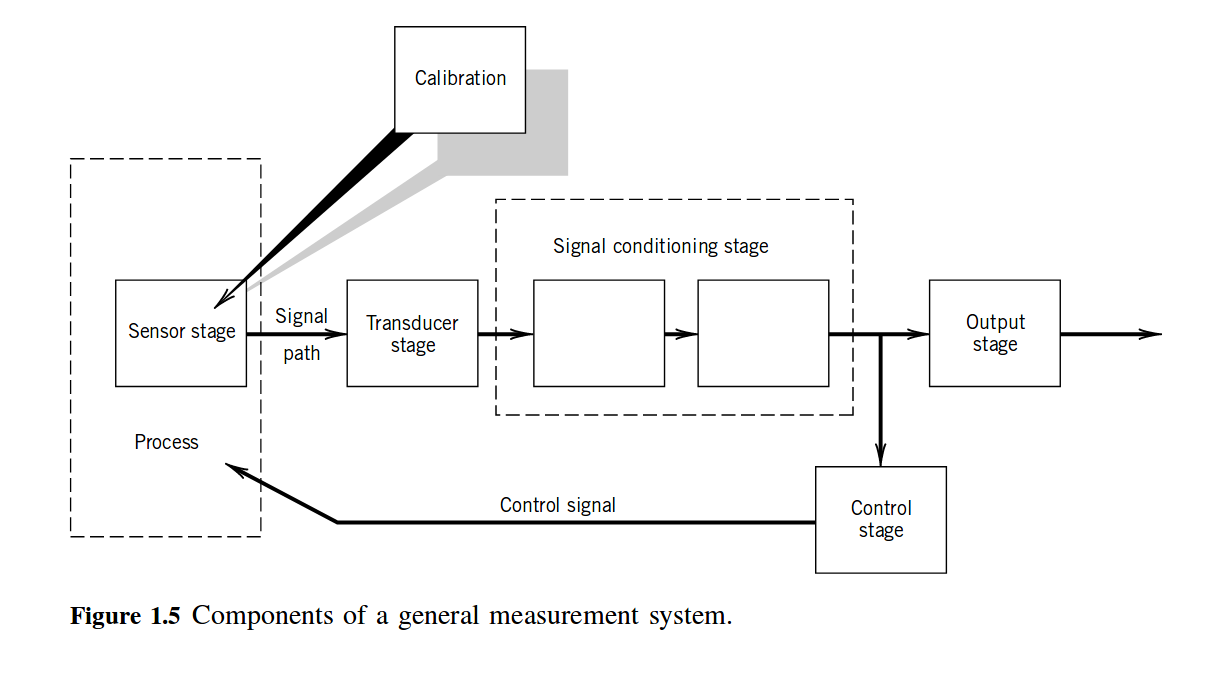
\includegraphics[scale=0.20]{images/measurement_stages.png}

				\btVFill
				{\tiny Image: Theory and Design of Mech. Meas.}

			\end{frame}

			\begin{frame}
				\frametitle{\sectionIsubsectionItitle}

				Sensors are typically classified as either {\bf analog} or {\bf digital} based on the type of signal that is output from the sensor. \vspace{5mm} \\

				
				However, this can be a misleading term. Many digital sensors operate based on analog circuit principles but require a digital circuit or MCU to operate or comminicate. \vspace{5mm} \\

				\begin{tabular}{|c|c|c|} \hline
				 	Analog \hspace*{10mm}& Digital \hspace*{10mm}& Both? \hspace*{10mm} \\ \hline   
				\end{tabular}	


			\end{frame}

			\begin{frame}
				\frametitle{\sectionIsubsectionItitle}

				Other Classifications:
				\begin{itemize}
					\item Contact vs Non-Contact

					\item Programmable (Configurable) vs Non-Programmable

					\item By Measured Variable	

				\end{itemize}


			\end{frame}

		% section I subsection II
		\subsection{\sectionIsubsectionIItitle}\label{sectionIsubsectionII}

			\begin{frame}
				\frametitle{\sectionIsubsectionIItitle}

				{\bf Thought Exercise:} How do we measure {\BL distance} (aka range)?        
	
					\begin{itemize}
					
						\item What variable or quantity is used to describe {\BL distance}?                         
						\begin{itemize}
							\item
							\item
							\item	
						\end{itemize} \vspace{5mm}
						\item What type of sensor is used to measure this?
						\begin{itemize}
							\item
							\item
							\item	
						\end{itemize}	

					\end{itemize}
				
				\btVFill

			\end{frame}

		

			\begin{frame}
				\frametitle{\sectionIsubsectionIItitle}


				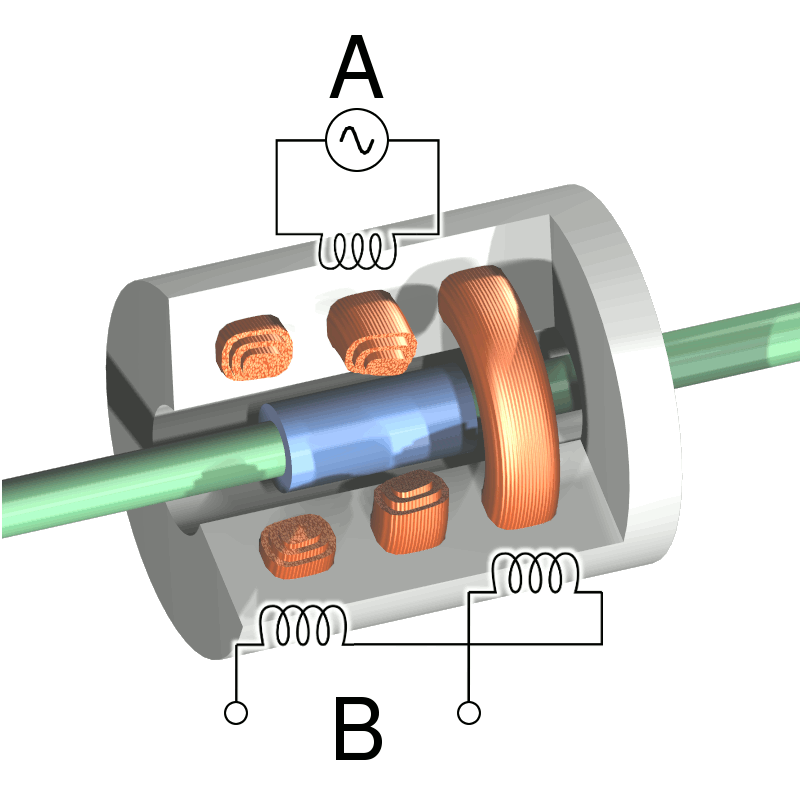
\includegraphics[scale=.2]{images/LVDT.png}

			 	\href{https://www.ni.com/en-us/innovations/white-papers/06/measuring-position-and-displacement-with-lvdts.html}{LVDTs with NI}\\
			 	\href{https://www.rdpe.com/us/hiw-lvdt.htm}{LVDT Animation}

			 	\btVFill
		
			\end{frame}

			\begin{frame}
				\frametitle{\sectionIsubsectionIItitle}
				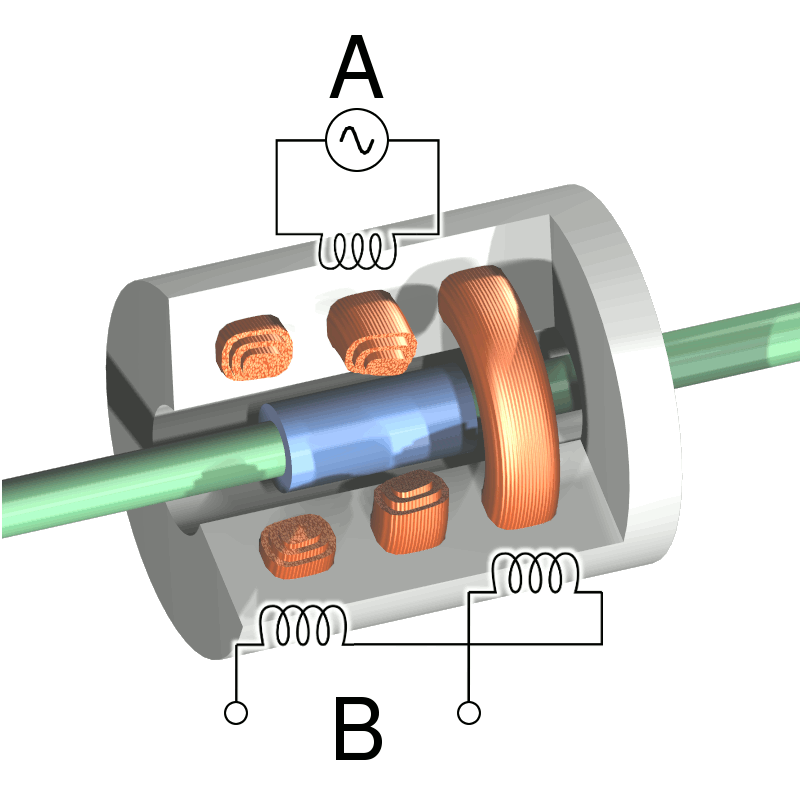
\includegraphics[scale=.2]{images/LVDT.png}
				\btVFill
			\end{frame}


			\begin{frame}
				\frametitle{\sectionIsubsectionIVtitle}

				\begin{itemize}
					\item What applications require this type of sensor?
					\begin{itemize}
						\item \vspace{5mm}
						\item \vspace{5mm}
						\item \vspace{5mm}	
					\end{itemize}
				\end{itemize}
				
				\btVFill
			\end{frame}

			\begin{frame}
				\frametitle{\sectionIsubsectionIVtitle}
				\begin{itemize}
					\item How does this type of sensor work?
					\begin{itemize}
						\item \vspace{5mm}
						\item \vspace{5mm}
						\item \vspace{5mm}	
					\end{itemize}
				\end{itemize}
				
				\btVFill

			\end{frame}


		% section I subsection III
		\subsection{\sectionIsubsectionIIItitle}\label{sectionIsubsectionIII}
			\begin{frame} 
				\frametitle{\sectionIsubsectionIIItitle}

				{\bf Thought Exercise:} How do we measure {\BL rotation}?        
	
					\begin{itemize}
					
						\item What variable or quantity is used to describe {\BL rotation}?                         
						\begin{itemize}
							\item
							\item
							\item	
						\end{itemize} \vspace{5mm}
						\item What type of sensor is used to measure this?
						\begin{itemize}
							\item
							\item
							\item	
						\end{itemize}	

					\end{itemize}
				
				\btVFill
			  
				
			\end{frame}	

			\begin{frame} 
				\frametitle{\sectionIsubsectionIIItitle}

				Rotational Potentiometer 

				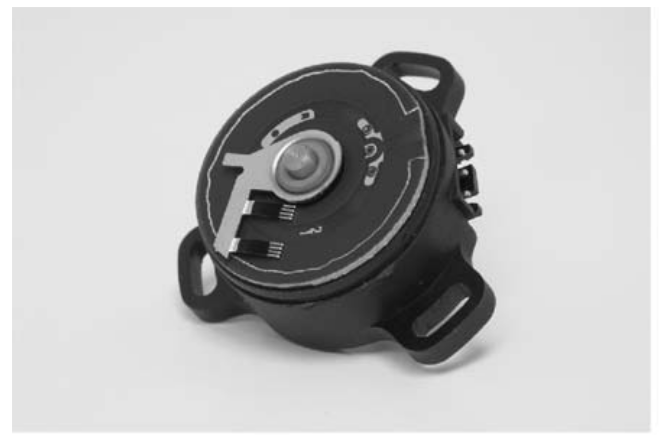
\includegraphics[scale=.25]{images/rot_pot.png}

				\btVFill	

			\end{frame}	

			\begin{frame}
				\frametitle{\sectionIsubsectionIIItitle}

				Absolute Encoder  
	
				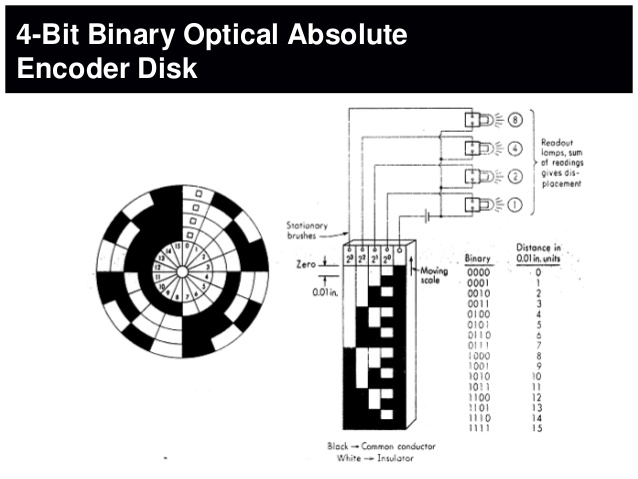
\includegraphics[scale=.35]{images/lecture1_fig1.jpg}	
				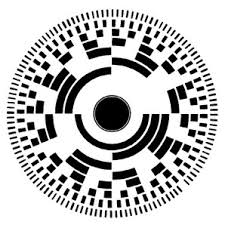
\includegraphics[scale=.25]{images/lecture1_fig2.jpg}

				\btVFill
				
			\end{frame}

			\begin{frame}

				Incremental Encoder  
	
				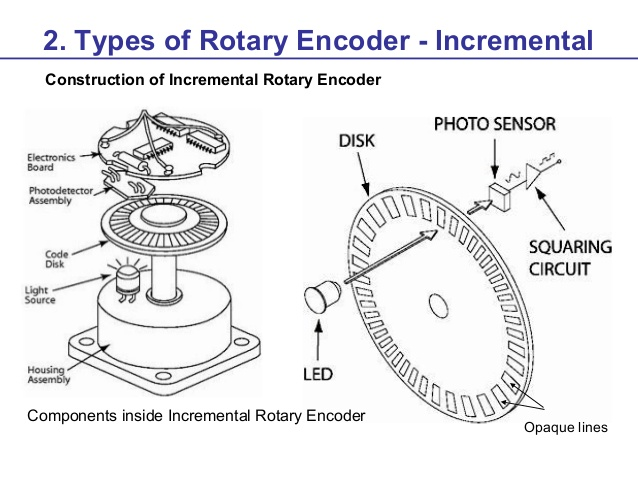
\includegraphics[scale=.35]{images/lecture1_fig3.jpg}	
	

				\btVFill
			\end{frame}


			\begin{frame}
				\frametitle{\sectionIsubsectionIIItitle}

				\begin{itemize}
					\item What applications require this type of sensor?
					\begin{itemize}
						\item \vspace{5mm}
						\item \vspace{5mm}
						\item \vspace{5mm}	
					\end{itemize}
				\end{itemize}

				\btVFill

			\end{frame}


			\begin{frame}
				\frametitle{\sectionIsubsectionIIItitle}

				\begin{itemize}
					\item How does this type of sensor work?
					\begin{itemize}
						\item \vspace{5mm}
						\item \vspace{5mm}
						\item \vspace{5mm}	
					\end{itemize}
				\end{itemize}
				
				\btVFill

			\end{frame}	

		% section I subsection IV
		\subsection{\sectionIsubsectionIVtitle}\label{sectionIsubsectionIV}		

			\begin{frame}
				\frametitle{\sectionIsubsectionIVtitle}
				{\bf Thought Exercise:} How do we measure {\PR orientation}?        
	
				\begin{itemize}
					
					\item What variable or quantity is used to describe {\PR orientation}?                         
					\begin{itemize}
						\item
						\item
						\item	
					\end{itemize} \vspace{5mm}
					\item What type of sensor is used to measure this?
					\begin{itemize}
						\item
						\item
						\item	
					\end{itemize}	
					
				\end{itemize}
				
				\btVFill
	
			\end{frame}

			\begin{frame}
				\frametitle{\sectionIsubsectionIVtitle}
				ADD EXAMPLE ORIENTATION SENSOR HERE

			\end{frame}

			\begin{frame}
				\frametitle{\sectionIsubsectionIVtitle}

				\begin{itemize}
					\item What applications require this type of sensor?
					\begin{itemize}
						\item \vspace{5mm}
						\item \vspace{5mm}
						\item \vspace{5mm}	
					\end{itemize}
				\end{itemize}
				
				\btVFill
			\end{frame}

			\begin{frame}
				\frametitle{\sectionIsubsectionIVtitle}
				\begin{itemize}
					\item How does this type of sensor work?
					\begin{itemize}
						\item \vspace{5mm}
						\item \vspace{5mm}
						\item \vspace{5mm}	
					\end{itemize}
				\end{itemize}
				
				\btVFill

			\end{frame}

	
	% Section II
	\section{\sectionIItitle}\label{sectionII}

		% section II Outline
		\begin{frame}
			\large \textbf{Topic 2 - \sectionIItitle} \vspace{3mm}\\

			\begin{itemize}
				\item \hyperlink{sectionIIsubsectionI}{\sectionIIsubsectionItitle} \vspc %  section II subsection I
				\item \hyperlink{sectionIIsubsectionII}{\sectionIIsubsectionIItitle} \vspc % section II subsection II
				\item \hyperlink{sectionIIsubsectionIII}{\sectionIIsubsectionIIItitle} \vspc % section II subsection III
				\item \hyperlink{sectionIIsubsectionIV}{\sectionIIsubsectionIVtitle} \vspc % section II subsection IV
			\end{itemize}

		\end{frame}

		% section II subsection I
		\subsection{\sectionIIsubsectionItitle}\label{sectionIIsubsectionI}

			\begin{frame}[label=sectionIIsubsectionI]
				\frametitle{\sectionIIsubsectionItitle}

				An integrated circuit (also known as an IC, a chip, or a microchip) is a set of electronic circuits on one small flat piece[a] of semiconductor material, usually silicon. Large numbers of miniaturized transistors and other electronic components are integrated together on the chip.	

				\btVFill
				{\tiny\href{https://en.wikipedia.org/wiki/Integrated_circuit}{wikipedia: integrated circuit}}
				
			\end{frame}	


			\begin{frame}[label=sectionIIsubsectionI]
				\frametitle{\sectionIIsubsectionItitle}	

				{\textbf Actvitity:} Group Brainstorming \\
				List three applications or devices that use ICs and or IC based sensors.
				\begin{itemize}
					\item
					\item
					\item
				\end{itemize}


				\btVFill	

			\end{frame}

		    \begin{frame}[label=sectionIIsubsectionI]
				\frametitle{\sectionIIsubsectionItitle}

				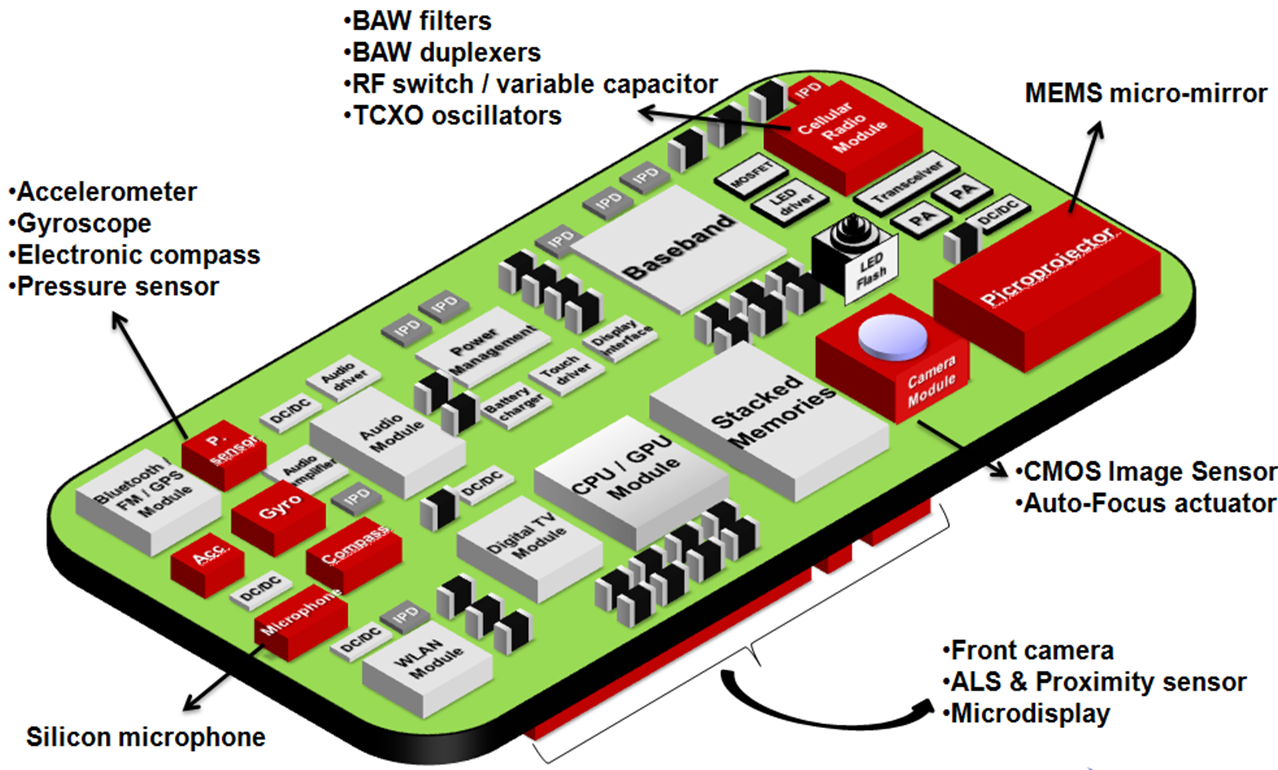
\includegraphics[scale=0.45]{images/Mobile_Device_Sensors.png}
	
				\btVFill	
		
			\end{frame}	

		% section II subsection II
		\subsection{\sectionIIsubsectionIItitle}\label{sectionIIsubsectionII}

			\begin{frame}
				\frametitle{\sectionIIsubsectionIItitle}
				
				MEMS (micro-electromechanical systems) is the technology of microscopic devices incorporating both electronic and moving parts. MEMS are made up of components between 1 and 100 micrometres in size (i.e., 0.001 to 0.1 mm), and MEMS devices generally range in size from 20 micrometres to a millimetre (i.e., 0.02 to 1.0 mm), although components arranged in arrays (e.g., digital micromirror devices) can be more than 1000 mm2.[1] They usually consist of a central unit that processes data (an integrated circuit chip such as microprocessor) and several components that interact with the surroundings (such as microsensors)
			
				\btVFill
				{\tiny \href{https://en.wikipedia.org/wiki/MEMS}{Wikipedia: MEMS}}

			\end{frame}

			\begin{frame}
				\frametitle{\sectionIIsubsectionIItitle}


				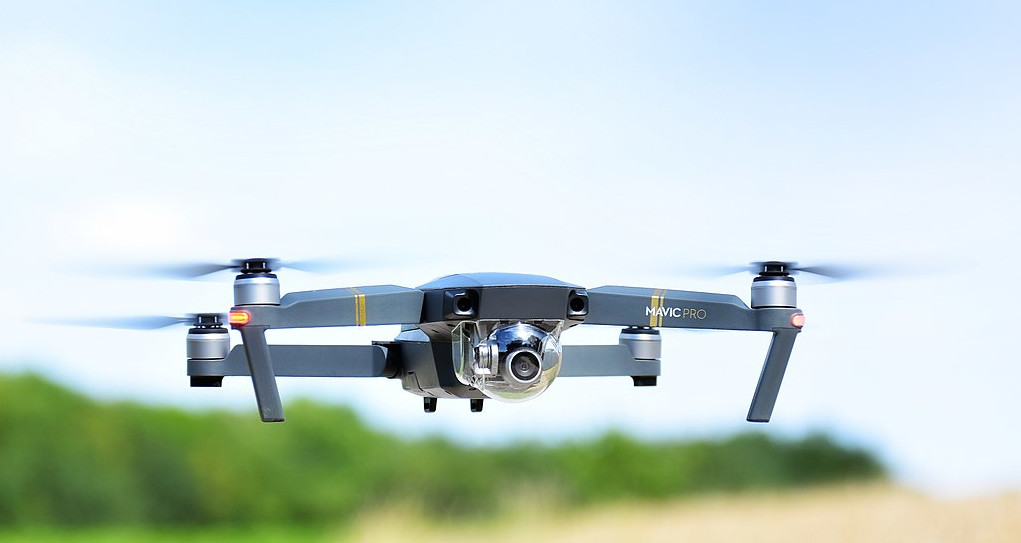
\includegraphics[scale=0.2]{images/Flying_DJI_Mavic_Pro_cropped.jpg}
	
				{\textbf Actvitity:} Group Brainstorming
				List three sensors that are found on a high performance quadcopter or drone.
				\begin{itemize}
					\item
					\item
					\item
				\end{itemize} 

			 	\btVFill


			\end{frame}



		% section II subsection III
		\subsection{\sectionIIsubsectionIIItitle}\label{sectionIIsubsectionIII}

			\begin{frame}
				\frametitle{\sectionIIsubsectionIIItitle}
				An accelerometer is a tool that measures proper acceleration, which is the acceleration of a body in its own instantaneous frame.

				Applications:
				\begin{itemize}
					\item Navigation Systems - Robotics - Aircraft - Missiles
					\item Personal Devices - Phones - Tablets
					\item Others:
				\end{itemize}                                

				\btVFill
				
			\end{frame}

			\begin{frame}
				\frametitle{\sectionIIsubsectionIIItitle}

			 	Thought Exercise: How do we measure acceleration? \vspace{10mm}\\                      
	
			 	{\textbf Actvitity:} Group Brainstorming \\
				Explain one method for measuring acceleration of a body.

			    \btVFill

			\end{frame}

			\begin{frame}
			\frametitle{\sectionIIsubsectionIIItitle}

				Mechanical Accelerometers Consist of a damped mass spring system and a sensing device.
	
			 	Types of accelerometers:

			 	\begin{itemize}
			 		
			 		\item Seismometer or Seismograph

			 		\item piezoelectric - charge in material resulting from mechanical stress

			 		\item piezoresistive - change in resistance resulting from mechanical stress

			 		\item capacitive 

			 	\end{itemize}

			 
			    \btVFill

			\end{frame}

			\begin{frame}
			\frametitle{\sectionIIsubsectionIIItitle}

				piezoelectric accelerometer                                
 
			 	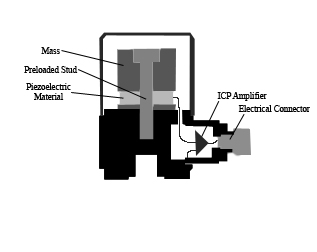
\includegraphics[scale=3.5]{images/PiezoAccel.jpg} 
			 	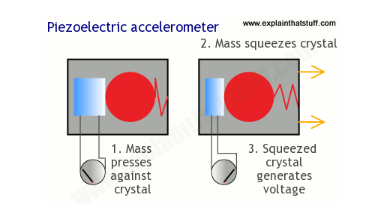
\includegraphics[scale=.55]{images/Piezoelectric.png}
			    \btVFill

			\end{frame}

			\begin{frame}
			\frametitle{\sectionIIsubsectionIIItitle}

				capacitive accelerometer                                
 
			 	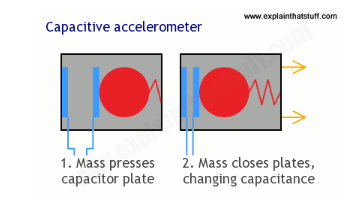
\includegraphics[scale=.55]{images/Capacitance.png}
			    \btVFill

			\end{frame}

		% section II subsection IV 
		\subsection{\sectionIIsubsectionIVtitle}\label{sectionIIsubsectionIV}

			\begin{frame}
				\frametitle{\sectionIIsubsectionIVtitle}

					{\bf Thought Exercise:} How do we measure {\BL orientation}?        
	
					\begin{itemize}
					
						\item What variable or quantity is used to describe motion?                         
						\begin{itemize}
							\item
							\item
							\item	
						\end{itemize} \vspace{5mm}
						\item What type of sensor is used to measure this?
						\begin{itemize}
							\item
							\item
							\item	
						\end{itemize}	

					\end{itemize}
				
				\btVFill


			\end{frame}

			\begin{frame}
				\frametitle{\sectionIIsubsectionIVtitle}

				\begin{itemize}
					\item What applications require this type of sensor?
					\begin{itemize}
						\item \vspace{5mm}
						\item \vspace{5mm}
						\item \vspace{5mm}	
					\end{itemize}
				\end{itemize}

				\btVFill	

			\end{frame}

			\begin{frame}
				\frametitle{\sectionIIsubsectionIVtitle}

				A magnetometer is a device that measures magnetic field or magnetic dipole moment. Different types of magnetometers measure the direction, strength, or relative change of a magnetic field at a particular location. A compass is one such device, one that measures the direction of an ambient magnetic field, in this case, the Earth's magnetic field. Other magnetometers measure the magnetic dipole moment of a magnetic material such as a ferromagnet, for example by recording the effect of this magnetic dipole on the induced current in a coil. 


				\btVFill	
				{\tiny \href{https://en.wikipedia.org/wiki/Magnetometer}{wikipedia: magnetometer} }

			\end{frame}
		
	
\end{document}

